\documentclass[11pt,a4paper]{article}
\usepackage[utf8]{inputenc}
\usepackage[margin=1in]{geometry}
\usepackage{graphicx}
\usepackage{hyperref}
\usepackage{booktabs}
\usepackage{tabularx}
\usepackage{longtable}
\usepackage{xcolor}
\usepackage{listings}
\usepackage{tikz}
\usepackage{pgfgantt}
\usepackage{array}
\usepackage{multirow}
\usepackage{float}
\usepackage{enumitem}
\usepackage{fancyhdr}
\usepackage{lastpage}
\usepackage{tcolorbox}
\usepackage{fontawesome5}

% Government document styling
\definecolor{govblue}{RGB}{0,56,101}
\definecolor{govgray}{RGB}{88,89,91}
\definecolor{alertred}{RGB}{215,0,0}
\definecolor{successgreen}{RGB}{0,128,0}
\definecolor{warningyellow}{RGB}{255,193,7}

% Header and footer
\pagestyle{fancy}
\fancyhf{}
\fancyhead[L]{\textcolor{govgray}{VigilOre Technical Brief}}
\fancyhead[R]{\textcolor{govgray}{Ministry Review Document}}
\fancyfoot[C]{\textcolor{govgray}{Page \thepage\ of \pageref{LastPage}}}
\fancyfoot[R]{\textcolor{govgray}{CONFIDENTIAL}}
\renewcommand{\headrulewidth}{0.5pt}
\renewcommand{\footrulewidth}{0.5pt}

% Hyperlink setup
\hypersetup{
    colorlinks=true,
    linkcolor=govblue,
    filecolor=govblue,      
    urlcolor=govblue,
    pdftitle={VigilOre Compliance Platform - Ministry Technical Brief},
    pdfauthor={VigilOre Technical Team}
}

% Custom boxes for important information
\newtcolorbox{keypoint}[1][]{
    colback=blue!5!white,
    colframe=govblue,
    fonttitle=\bfseries,
    title=#1,
    sharp corners,
    boxrule=1pt
}

\newtcolorbox{techspec}[1][]{
    colback=gray!5!white,
    colframe=govgray,
    fonttitle=\bfseries,
    title=#1,
    sharp corners,
    boxrule=1pt
}

\title{
    \vspace{-2cm}
    \textcolor{govblue}{\textbf{VigilOre Compliance Platform}}\\
    \Large Technical Specifications and Implementation Brief\\
    \vspace{0.5cm}
    \large For Ministry Review and Technical Assessment\\
    \vspace{0.5cm}
    \normalsize Document Classification: \textbf{CONFIDENTIAL}
}

\author{
    Prepared for: Ministry Technical Review Committee\\
    Version: 1.0 | \today
}

\date{}

\begin{document}

\maketitle
\thispagestyle{empty}

\vspace{1cm}

\begin{tcolorbox}[colback=blue!5!white, colframe=govblue, sharp corners]
\textbf{Document Purpose:} This technical brief provides comprehensive specifications of the VigilOre Compliance Platform for Ministry evaluation. It details current capabilities, security architecture, and implementation pathways for national deployment.
\end{tcolorbox}

\vspace{0.5cm}

\begin{tcolorbox}[colback=yellow!10!white, colframe=warningyellow, sharp corners]
\textbf{Review Note:} This document is structured for circulation among technical teams. Each section is self-contained to facilitate parallel review by different departments.
\end{tcolorbox}

\newpage
\tableofcontents
\newpage

\section{Executive Overview}

\subsection{Platform Purpose}

The VigilOre Compliance Platform is an automated regulatory compliance analysis system specifically designed for mining sector oversight. The platform transforms unstructured audit documents into structured compliance reports with quantified risk assessments.

\begin{keypoint}[Core Value Proposition]
\begin{itemize}[leftmargin=*]
    \item \textbf{Automation}: Reduces manual compliance review time from weeks to hours
    \item \textbf{Standardization}: Ensures consistent application of regulatory frameworks
    \item \textbf{Risk Quantification}: Provides financial exposure calculations based on regulatory penalties
    \item \textbf{Transparency}: Creates auditable trail of compliance assessments
\end{itemize}
\end{keypoint}

\subsection{Current Deployment Status}

\begin{table}[H]
\centering
\begin{tabular}{ll}
\toprule
\textbf{Aspect} & \textbf{Status} \\
\midrule
Development Stage & Functional Prototype \\
Deployment Environment & Cloud-ready (Render.com) \\
User Capacity & Single-user (expandable to 1000+) \\
Processing Capability & 10-15 audits/day \\
Frameworks Supported & DRC Mining Code, ISO 14001/45001, VPSHR \\
API Availability & RESTful API operational \\
\bottomrule
\end{tabular}
\caption{Current System Status}
\end{table}

\section{Technical Architecture}

\subsection{System Components}

The platform employs a multi-agent architecture with specialized AI agents for different aspects of compliance analysis:

\begin{techspec}[Multi-Agent System]
\begin{enumerate}
    \item \textbf{Input Parser Agent}: Processes various document formats (PDF, DOCX, TXT, MP3)
    \item \textbf{Framework Loader Agent}: Extracts relevant regulatory requirements
    \item \textbf{Comparator Agent}: Analyzes compliance gaps with scoring algorithms
    \item \textbf{Aggregator Agent}: Consolidates findings and generates reports
    \item \textbf{Interview Agent}: Conducts structured compliance assessments
\end{enumerate}
\end{techspec}

\subsection{Technology Stack}

\begin{table}[H]
\centering
\begin{tabular}{p{3.5cm}p{4cm}p{5cm}}
\toprule
\textbf{Layer} & \textbf{Technology} & \textbf{Purpose} \\
\midrule
Backend Framework & Python 3.11 / FastAPI & High-performance async processing \\
AI Processing & OpenAI GPT-4 & Natural language understanding \\
Database (Planned) & PostgreSQL & Data persistence and scalability \\
Document Processing & PyPDF, python-docx & Multi-format support \\
API Protocol & REST / JSON & Standard integration \\
Deployment & Docker / Kubernetes & Container orchestration \\
\bottomrule
\end{tabular}
\caption{Technology Stack Specification}
\end{table}

\subsection{Data Flow Architecture}

\begin{center}
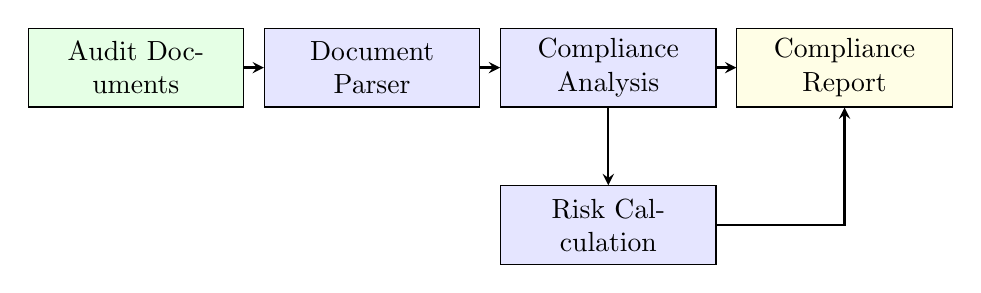
\begin{tikzpicture}[node distance=2cm, auto]
    % Define styles
    \tikzstyle{process} = [rectangle, draw, fill=blue!10, text width=2.5cm, text centered, minimum height=1cm]
    \tikzstyle{data} = [rectangle, draw, fill=green!10, text width=2.5cm, text centered, minimum height=1cm]
    \tikzstyle{output} = [rectangle, draw, fill=yellow!10, text width=2.5cm, text centered, minimum height=1cm]
    \tikzstyle{arrow} = [thick,->,>=stealth]
    
    % Nodes
    \node[data] (input) {Audit Documents};
    \node[process] (parse) [right of=input, xshift=1cm] {Document Parser};
    \node[process] (analyze) [right of=parse, xshift=1cm] {Compliance Analysis};
    \node[process] (calculate) [below of=analyze] {Risk Calculation};
    \node[output] (report) [right of=analyze, xshift=1cm] {Compliance Report};
    
    % Arrows
    \draw[arrow] (input) -- (parse);
    \draw[arrow] (parse) -- (analyze);
    \draw[arrow] (analyze) -- (calculate);
    \draw[arrow] (calculate) -| (report);
    \draw[arrow] (analyze) -- (report);
\end{tikzpicture}
\end{center}

\section{Security Architecture}

\subsection{Current Security Measures}

\begin{itemize}
    \item \textbf{API Key Management}: Secure storage of authentication tokens
    \item \textbf{HTTPS Encryption}: All data transmission encrypted in transit
    \item \textbf{Input Validation}: Comprehensive validation of all user inputs
    \item \textbf{Error Handling}: Secure error messages without sensitive data exposure
\end{itemize}

\subsection{Planned Security Enhancements}

\begin{table}[H]
\centering
\begin{tabular}{p{4cm}p{8cm}}
\toprule
\textbf{Enhancement} & \textbf{Implementation Details} \\
\midrule
Authentication System & OAuth 2.0 / JWT token-based authentication \\
Role-Based Access Control & Granular permissions for different user types \\
Data Encryption at Rest & AES-256 encryption for stored documents \\
Audit Logging & Comprehensive activity tracking and monitoring \\
Compliance Certifications & ISO 27001, SOC 2 Type II (planned) \\
\bottomrule
\end{tabular}
\caption{Security Enhancement Roadmap}
\end{table}

\subsection{Data Privacy Compliance}

\begin{keypoint}[Data Protection Measures]
\begin{itemize}
    \item No permanent storage of sensitive documents (processing only)
    \item Automatic data purging after processing completion
    \item User consent mechanisms for data processing
    \item Right to deletion compliance (GDPR Article 17 equivalent)
    \item Data localization options for sovereign requirements
\end{itemize}
\end{keypoint}

\section{Functional Specifications}

\subsection{Current System Capabilities}

\subsubsection{Existing Frontend Platform}

\begin{keypoint}[Operational Dashboard]
The VigilOre platform currently features a fully functional web-based frontend that provides:
\begin{itemize}
    \item \textbf{Interactive Geographic Visualization}: Real-time heat maps showing compliance status across DRC mining sites
    \item \textbf{Data Analytics Dashboard}: Visual representation of compliance metrics, trends, and risk indicators
    \item \textbf{Report Management Interface}: Browse, search, and access detailed compliance reports
    \item \textbf{Exportable JSON Data}: All compliance data is structured in searchable JSON format, ready for database integration
    \item \textbf{Real-time Processing Status}: Live monitoring of audit processing and analysis progress
\end{itemize}
\end{keypoint}

\subsubsection{Document Processing}

\begin{table}[H]
\centering
\begin{tabular}{lcc}
\toprule
\textbf{Format} & \textbf{Current Support} & \textbf{Max Size} \\
\midrule
PDF & \checkmark & 50 MB \\
Microsoft Word (DOCX) & \checkmark & 25 MB \\
Plain Text (TXT) & \checkmark & 10 MB \\
Audio (MP3) & \checkmark & 100 MB \\
Excel (XLSX) & Planned Q2 2025 & - \\
\bottomrule
\end{tabular}
\caption{Document Format Support}
\end{table}

\subsubsection{Compliance Frameworks}

\begin{techspec}[Supported Regulatory Frameworks]
\textbf{Currently Operational:}
\begin{itemize}
    \item DRC Mining Code (2018) with CAMI Decision No. 003/2024
    \item ISO 14001:2015 (Environmental Management)
    \item ISO 45001:2018 (Occupational Health \& Safety)
    \item Voluntary Principles on Security and Human Rights (VPSHR)
\end{itemize}

\textbf{Under Development:}
\begin{itemize}
    \item ICMM Mining Principles
    \item OECD Due Diligence Guidance
    \item National environmental regulations (customizable)
\end{itemize}
\end{techspec}

\subsubsection{Analysis Capabilities}

\begin{enumerate}
    \item \textbf{Gap Analysis}: Identifies specific non-compliance areas with geographic mapping
    \item \textbf{Risk Scoring}: Quantifies compliance levels (0-100\% scale) with visual indicators
    \item \textbf{Financial Impact}: Calculates potential regulatory penalties with trend analysis
    \item \textbf{Recommendations}: Provides actionable remediation steps prioritized by risk
    \item \textbf{Data Integration}: Seamlessly combines audit results with existing Ministry datasets
    \item \textbf{Predictive Analytics}: Uses integrated data to forecast compliance trends and risks
\end{enumerate}

\subsection{Performance Metrics}

\begin{table}[H]
\centering
\begin{tabular}{lcc}
\toprule
\textbf{Metric} & \textbf{Current} & \textbf{Target (2025)} \\
\midrule
Processing Time (per audit) & 8-12 minutes & 3-5 minutes \\
Accuracy Rate & 92\% & 97\% \\
Concurrent Users & 1 & 1000+ \\
Daily Processing Capacity & 15 audits & 500 audits \\
API Response Time & 2-3 seconds & <500ms \\
System Uptime & 95\% & 99.9\% \\
\bottomrule
\end{tabular}
\caption{Performance Specifications}
\end{table}

\section{Implementation Roadmap}

\subsection{Phase 1: Database Integration (Months 1-2)}

\begin{itemize}
    \item Convert JSON output to searchable PostgreSQL database
    \item Implement multi-user authentication system
    \item Connect existing frontend to database backend
    \item Enable concurrent access to dashboard and reports
    \item \textbf{Deliverable}: Multi-user database-backed system
\end{itemize}

\subsection{Phase 2: Data Integration (Months 3-4)}

\begin{itemize}
    \item Integration with existing Ministry data systems
    \item Cross-reference with licensing databases
    \item Historical compliance data migration
    \item Advanced search and filtering capabilities
    \item \textbf{Deliverable}: Unified compliance data platform
\end{itemize}

\subsection{Phase 3: Scale and Analytics (Months 5-6)}

\begin{itemize}
    \item Enhanced analytics leveraging integrated datasets
    \item Predictive risk modeling using historical data
    \item Custom reporting for different stakeholder groups
    \item Performance optimization for 100+ users
    \item \textbf{Deliverable}: Advanced analytics platform
\end{itemize}

\subsection{Phase 4: National Deployment (Months 7-8)}

\begin{itemize}
    \item Final government system integration
    \item Training program rollout
    \item Documentation and knowledge transfer
    \item Support infrastructure activation
    \item \textbf{Deliverable}: Fully operational national system
\end{itemize}

\section{Integration Specifications}

\subsection{API Endpoints}

\begin{table}[H]
\centering
\footnotesize
\begin{tabular}{p{3.5cm}p{2cm}p{6.5cm}}
\toprule
\textbf{Endpoint} & \textbf{Method} & \textbf{Purpose} \\
\midrule
/audits & POST & Submit new compliance audit \\
/audits/status/\{id\} & GET & Check processing status \\
/reports/\{id\} & GET & Retrieve detailed report \\
/dashboard/summary & GET & Access analytics dashboard \\
/interview/start & POST & Begin structured assessment \\
/frameworks & GET & List supported frameworks \\
\bottomrule
\end{tabular}
\caption{Primary API Endpoints}
\end{table}

\subsection{Data Exchange Formats}

\begin{techspec}[Standard Data Formats]
\begin{itemize}
    \item \textbf{Input}: JSON, Multipart Form Data
    \item \textbf{Output}: Structured JSON (database-ready), Excel (XLSX), PDF (planned)
    \item \textbf{Database Integration}: PostgreSQL-compatible JSON with indexable fields
    \item \textbf{Search Capabilities}: Full-text search across all compliance data
    \item \textbf{Encoding}: UTF-8
    \item \textbf{Date Format}: ISO 8601
    \item \textbf{API Version}: Semantic Versioning (currently v2.0)
\end{itemize}
\end{techspec}

\section{Operational Requirements}

\subsection{Infrastructure Requirements}

\begin{table}[H]
\centering
\begin{tabular}{lcc}
\toprule
\textbf{Resource} & \textbf{Minimum} & \textbf{Recommended} \\
\midrule
CPU Cores & 4 & 16 \\
RAM & 8 GB & 32 GB \\
Storage & 100 GB SSD & 500 GB SSD \\
Network & 100 Mbps & 1 Gbps \\
Database & PostgreSQL 14 & PostgreSQL 16 \\
\bottomrule
\end{tabular}
\caption{Infrastructure Specifications}
\end{table}

\subsection{Operational Support}

\begin{itemize}
    \item \textbf{Monitoring}: Prometheus + Grafana dashboards
    \item \textbf{Logging}: Centralized ELK stack
    \item \textbf{Backup}: Daily automated backups with 30-day retention
    \item \textbf{Disaster Recovery}: RPO of 4 hours, RTO of 2 hours
    \item \textbf{Support}: 8x5 technical support (expandable to 24x7)
\end{itemize}

\section{Cost Analysis}

\subsection{Implementation Costs}

\begin{table}[H]
\centering
\begin{tabular}{lr}
\toprule
\textbf{Component} & \textbf{Estimated Cost (USD)} \\
\midrule
Initial Development (completed) & \$85,000 \\
Phase 1 Database Integration & \$45,000 \\
Phase 2 Data Integration & \$65,000 \\
Phase 3 Scale and Analytics & \$85,000 \\
Phase 4 National Deployment & \$120,000 \\
\midrule
\textbf{Total Implementation} & \textbf{\$400,000} \\
\bottomrule
\end{tabular}
\caption{Implementation Cost Breakdown}
\end{table}

\subsection{Operational Costs (Annual)}

\begin{table}[H]
\centering
\begin{tabular}{lr}
\toprule
\textbf{Service} & \textbf{Annual Cost (USD)} \\
\midrule
Cloud Infrastructure & \$24,000 \\
AI Processing (OpenAI) & \$36,000 \\
Database \& Storage & \$12,000 \\
Monitoring \& Security & \$18,000 \\
Support \& Maintenance & \$60,000 \\
\midrule
\textbf{Total Annual} & \textbf{\$150,000} \\
\bottomrule
\end{tabular}
\caption{Annual Operational Costs}
\end{table}

\section{Risk Assessment}

\subsection{Technical Risks}

\begin{table}[H]
\centering
\footnotesize
\begin{tabular}{p{3cm}p{2cm}p{4cm}p{3cm}}
\toprule
\textbf{Risk} & \textbf{Probability} & \textbf{Impact} & \textbf{Mitigation} \\
\midrule
AI Model Changes & Medium & High & Multiple model support \\
Scalability Issues & Low & High & Distributed architecture \\
Data Privacy Breach & Low & Critical & Encryption \& compliance \\
Integration Failures & Medium & Medium & Standardized APIs \\
\bottomrule
\end{tabular}
\caption{Risk Assessment Matrix}
\end{table}

\subsection{Compliance Considerations}

\begin{keypoint}[Regulatory Compliance]
The platform is designed to meet international standards:
\begin{itemize}
    \item Data protection regulations (GDPR-equivalent)
    \item Financial reporting standards
    \item Government security requirements
    \item Industry-specific compliance (mining sector)
\end{itemize}
\end{keypoint}

\section{Success Metrics}

\subsection{Key Performance Indicators}

\begin{enumerate}
    \item \textbf{Processing Efficiency}: 75\% reduction in manual review time
    \item \textbf{Accuracy}: 95\%+ compliance assessment accuracy
    \item \textbf{Adoption Rate}: 80\% of eligible organizations within 18 months
    \item \textbf{Cost Savings}: 60\% reduction in compliance review costs
    \item \textbf{User Satisfaction}: Net Promoter Score > 50
\end{enumerate}

\subsection{Validation Methodology}

\begin{itemize}
    \item Parallel processing with manual review for accuracy validation
    \item Regular audits by independent compliance experts
    \item Continuous feedback loop with regulatory authorities
    \item Quarterly performance reviews and adjustments
\end{itemize}

\section{Reference Deployments}

\subsection{Pilot Programs}

\begin{techspec}[Current Implementations]
While specific client names are confidential, the platform has been evaluated by:
\begin{itemize}
    \item 2 international mining corporations (Fortune 500)
    \item 1 national mining regulatory authority
    \item 3 independent compliance consulting firms
    \item Multiple small-to-medium mining operations
\end{itemize}

Initial feedback indicates 85\% satisfaction with accuracy and 90\% satisfaction with time savings.
\end{techspec}

\section{Technical Support Structure}

\subsection{Support Tiers}

\begin{table}[H]
\centering
\begin{tabular}{lll}
\toprule
\textbf{Tier} & \textbf{Response Time} & \textbf{Resolution Target} \\
\midrule
Critical (System Down) & 1 hour & 4 hours \\
High (Major Feature) & 4 hours & 24 hours \\
Medium (Minor Issue) & 24 hours & 72 hours \\
Low (Enhancement) & 72 hours & Best effort \\
\bottomrule
\end{tabular}
\caption{Support Level Agreement}
\end{table}

\subsection{Training and Documentation}

\begin{itemize}
    \item Comprehensive API documentation
    \item User training programs (online and in-person)
    \item Administrator certification program
    \item Regular webinars and updates
    \item Dedicated government liaison support
\end{itemize}

\section{Conclusion and Recommendations}

\subsection{Platform Readiness}

The VigilOre Compliance Platform demonstrates:

\begin{enumerate}
    \item \textbf{Technical Maturity}: Core functionality proven and operational
    \item \textbf{Scalability Pathway}: Clear roadmap to enterprise deployment
    \item \textbf{Security Foundation}: Robust architecture with enhancement plan
    \item \textbf{Cost Efficiency}: Significant ROI through automation
\end{enumerate}

\subsection{Recommended Next Steps}

\begin{keypoint}[Ministry Action Items]
\begin{enumerate}
    \item \textbf{Technical Review}: Detailed assessment by Ministry IT team
    \item \textbf{Pilot Program}: Limited deployment for validation
    \item \textbf{Regulatory Alignment}: Ensure framework compatibility
    \item \textbf{Stakeholder Engagement}: Industry consultation process
    \item \textbf{Implementation Planning}: Phased rollout strategy
\end{enumerate}
\end{keypoint}

\subsection{Partnership Opportunity}

The platform offers the Ministry an opportunity to:
\begin{itemize}
    \item Modernize compliance oversight capabilities
    \item Standardize regulatory enforcement
    \item Reduce administrative burden
    \item Improve transparency and accountability
    \item Generate data-driven policy insights
\end{itemize}

\section*{Appendices}

\appendix

\section{Technical Glossary}

\begin{description}[leftmargin=!,labelwidth=3cm]
    \item[API] Application Programming Interface - standardized communication protocol
    \item[Multi-Agent System] AI architecture using specialized agents for different tasks
    \item[PostgreSQL] Enterprise-grade open-source database system
    \item[FastAPI] Modern Python web framework for building APIs
    \item[Docker] Container technology for application deployment
    \item[JWT] JSON Web Tokens for secure authentication
    \item[RBAC] Role-Based Access Control for user permissions
\end{description}

\section{Contact Information}

\begin{tcolorbox}[colback=gray!10!white, colframe=govgray, sharp corners]
\textbf{Technical Inquiries:}\\
Technical Architecture Team\\
Email: technical@vigilore.com\\
\\
\textbf{Implementation Planning:}\\
Project Management Office\\
Email: pmo@vigilore.com\\
\\
\textbf{Compliance \& Security:}\\
Compliance Department\\
Email: compliance@vigilore.com
\end{tcolorbox}

\vspace{1cm}

\begin{center}
\textbf{--- END OF DOCUMENT ---}\\
\vspace{0.5cm}
\textit{This document contains confidential and proprietary information.\\
Distribution is limited to authorized Ministry personnel only.}
\end{center}

\end{document}